% Preamble
% ---
\documentclass[11pt,a4paper,english]{article}

% Packages
% ---
\usepackage{amsmath} % Advanced math typesetting
\usepackage[utf8]{inputenc} % Unicode support (Umlauts etc.)
\usepackage[english]{babel} % Change hyphenation rules
\usepackage{hyperref} % Add a link to your document
\usepackage{graphicx} % Add pictures to your document
\usepackage{listings} % Source code formatting and highlighting
\usepackage{makeidx}
\bibliographystyle{plain}

% ---
\begin{document}
\title{Synopsis}
\begin{titlepage}
    \begin{center}
        \LARGE
        \textbf{A Minor Project Synopsis}\\
        on\\
        \Huge
        \textbf{Chaos Based Image Encryption for Medical Reports}\\
        \vspace{0.5cm}
        \Large
        Submitted to Manipal University Jaipur\\
        towards the partial fulfillment for the award of the degree of\\
        \vspace{0.5cm}
        \LARGE
        \textbf{Bachelor of Technology}\\
        \textbf{In Information Technology}\\
        \vspace{0.5cm}
        \large
        By\\
        \Large
        \textbf{Ayush Jaipuriyar}\\
        209302167\\
        \textbf{Pratham Dhiman}\\
        209302249\\
        Section E\\
        \vspace{0.5cm}
        \large
        Under the Guidance of\\
        \Large
        \textbf{Dr. Anju Yadav }

        \vfill

        
\includegraphics[width=11.58cm,height=2.28cm]{./logo}

        \LARGE
        \textbf{Department of Information Technology}\\
        \textbf{School of Information Technology }\\
        \textbf{Manipal University Jaipur}\\
        \Large
        \textbf{2022-2023}

    \end{center}
\end{titlepage}
\newpage
\date{}
\title{}
\maketitle
\tableofcontents
\newpage
\section{Introduction}
Encryption of images is important in today's digital world as it helps to protect sensitive and confidential information contained in images from unauthorized access. With the increasing use of digital images for personal, business and government purposes, there is a growing need to ensure that this data is protected from hackers, cyber-criminals and other malicious actors who might use the information for their own purposes. Encryption provides a secure and effective means of protecting images by transforming them into an unreadable form, making it difficult for unauthorized individuals to access or view the original image. This helps to ensure the privacy and confidentiality of the information contained in the image and reduces the risk of data breaches and theft.
\subsection{Encryption}
Encryption is the process of converting plaintext into an unreadable form (ciphertext) to protect its confidentiality and prevent unauthorized access to its content. It uses mathematical algorithms (cipher) and a key to transform the data. Only those with the corresponding decryption key can reverse the process and access the original plaintext. Encryption helps to ensure the privacy and security of data transmitted over networks or stored on devices.
\subsection{Chaos Theory}
Chaos theory is a branch of mathematics that studies the behavior of dynamic systems that are highly sensitive to initial conditions, leading to seemingly random patterns and unpredictable behavior. It deals with how small differences in initial conditions can lead to vastly different outcomes over time, which is often referred to as the butterfly effect. Chaos theory has applications in various fields, such as physics, economics, and weather forecasting.

Chaos theory provides several important features to image encryption, including:
\begin{enumerate}
    \item \textbf{Sensitivity to Initial Conditions}: The sensitivity to initial conditions in chaotic systems provides a high degree of security as small differences in the initial conditions can lead to vastly different results, making it difficult for an attacker to determine the encryption process.
    \item \textbf{Unpredictability:} The unpredictable behavior of chaotic systems adds an extra layer of security as the encrypted image appears to be random noise, making it difficult for an attacker to determine the original image.
    \item \textbf{High-dimensional Dynamics:} The high-dimensional dynamics of chaotic systems allow for the creation of complex encryption algorithms that can provide a high degree of security.
    \item \textbf{Ease of Implementation:} The mathematical simplicity of some chaotic systems makes them easy to implement in software, providing a convenient means of encrypting images.
\end{enumerate}
Overall, chaos theory provides a means of creating secure, efficient, and easy-to-implement image encryption algorithms that can help protect sensitive information transmitted over communication networks.
\newpage
\section{Motivation}

Our motivation for developing a new chaos-based image encryption technique is a result of our passion for cryptography and our fascination with chaos theory. I believe that this research will not only advance the field of cryptography but also help to improve the security of sensitive information. The challenge of developing a new image encryption technique appeals to me and I am eager to explore the unique properties of chaos-based encryption and apply them to image encryption. This work presents a significant challenge and an opportunity for me to push the boundaries of what is currently possible. Successfully developing a new chaos-based image encryption technique would be a major accomplishment for me, both professionally and personally, and would be a source of pride and satisfaction in our career as a researcher.
\paragraph{}
\newpage
\section{Project Objectives}
\paragraph{}
The objectives of the project are out lined as follows :-
\begin{enumerate}
    \item To develop an efficient and secure image encryption system for medical images that meets the requirements of the hospital.

    \item To ensure the privacy and security of medical images and information stored and transmitted within the hospital network.

    \item To comply with relevant regulations and standards regarding the storage and transmission of medical information and images.

    \item To provide authorized personnel with fast and secure access to encrypted medical images.

    \item To improve the backup and recovery of medical images, ensuring that important information is not lost in case of data loss or corruption.

    \item To reduce the risk of data breaches and unauthorized access to sensitive medical information.

    \item To increase the efficiency and accuracy of medical diagnoses and treatment decisions by enabling fast and secure access to medical images.

    \item To provide a user-friendly interface for encrypting and decrypting medical images, with a focus on simplicity and ease of use.

    \item To ensure that the encryption system can scale to accommodate the growing needs of the hospital over time.\newpage
\end{enumerate}
\section{Methodology}
\paragraph{}
\begin{enumerate}
    \item Select a chaotic system: Choose a well-studied and well-understood chaotic system that can be used as the basis for the encryption algorithm. For example, the logistic map or the Lorenz system can be used.

    \item Generate a chaotic sequence: Using the selected chaotic system, generate a chaotic sequence that will be used as the key for the encryption process. The length of the sequence should be equal to or greater than the number of pixels in the image.

    \item Initialize encryption parameters: Select the encryption parameters such as the number of iterations, the number of encryption rounds, and the size of the encryption block. These parameters will determine the strength of the encryption.

    \item Divide the image into blocks: Divide the original image into smaller blocks of a fixed size. The size of the blocks should be selected to optimize the encryption process.

    \item Perform encryption: For each block of the image, perform the encryption process. The encryption process involves combining the block with the chaotic sequence using an appropriate encryption algorithm, such as XOR or addition. The encrypted block is then stored in a new image.

    \item Repeat encryption: Repeat the encryption process for each block of the image for the specified number of encryption rounds.

    \item Store the encrypted image: Store the encrypted image on a secure storage device, such as a hard drive or a secure cloud storage service. The original image and the encryption key should also be stored securely.

    \item Decryption process: To decrypt the image, the same encryption process is performed in reverse using the encryption key.
\end{enumerate}
\newpage
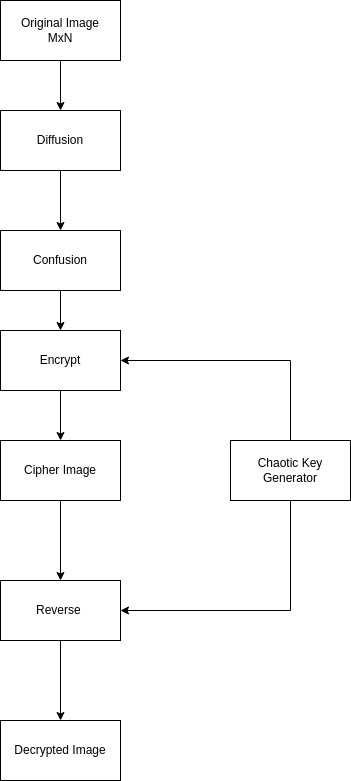
\includegraphics[height=18cm,width=15cm]{graph}
\newpage
\section{Facilties reqired for proposed work}
\subsection[short]{Hardware Requirements}
For an image encryption project that needs to be deployed in a hospital environment, the hardware requirements may need to be higher to ensure stability and performance. Here are some suggested hardware requirements:
\begin{enumerate}
    \item \textbf{Processor:} A high-performance processor with multiple cores and a high clock speed is recommended for fast processing and encryption of medical images.

    \item \textbf{RAM:} At least 16GB of RAM, but 32GB or more is recommended to ensure smooth processing of large medical images.But for now 4GB is also enough

    \item \textbf{Storage:} A solid-state drive (SSD) with a large capacity for storing encrypted medical images and other data.

    \item \textbf{Graphics Card:} A dedicated graphics card with a high amount of VRAM for rendering medical images in real-time.

    \item \textbf{Network Connectivity:} Fast and reliable network connectivity is essential for transferring medical images and other data within the hospital network.
\end{enumerate}
\subsection[short]{Software Requirements}
A few of the basic software requirements are as follows:-
\begin{enumerate}
    \item \textbf{Operating System:} Any modern operating system such as Windows, Linux, or macOS should suffice.

    \item \textbf{Programming Language:} Python

    \item \textbf{Image Processing Library:} An image processing library such as OpenCV, Pillow, or scikit-image for processing and manipulating images.

    \item \textbf{Development Environment:} An integrated development environment (IDE) such as Visual Studio Code for writing and testing code.

    \item \textbf{Version Control System:} A version control system such as Git for tracking changes and collaborating with others.

\end{enumerate}
\newpage
\section{Bibliography}
% \print
\bibliography{Synopsis}
\nocite{*}
\end{document}
